\documentclass{article}

\usepackage[latin1]{inputenc}
\usepackage{tikz}

\begin{document}
\pagestyle{empty}


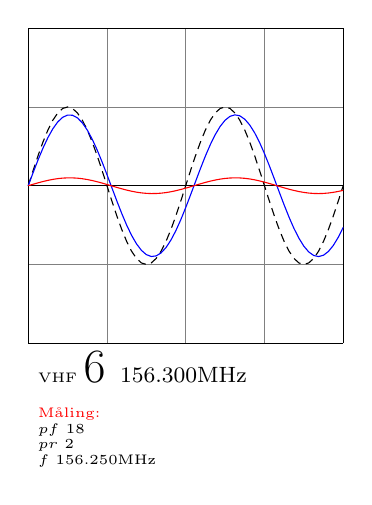
\begin{tikzpicture}[domain=0:4]
    \draw[very thin,color=gray] (0,-2) grid (4,2);
    \draw[-] (0,2) -- (4, 2);
    \draw[-] (4,2) -- (4, -2);
    \draw[-] (4,-2) -- (0, -2);
    \draw[-] (0,-2) -- (0, 2);
    \draw[-] (0,0) -- (4,0); 
    \draw[black, densely dashed, samples=65] plot (\x, {sin(pi*\x*1 r)});
    \draw[blue, samples=65] plot(\x, {(1/20)/(1/18)*sin(pi*\x*.950 r)});
    \draw[red, samples=65] plot(\x, {(1/20)/(1/2)*sin(pi*\x*.950 r)}); 
    \node[black, anchor=west] at (0,-2.3) {\tiny{VHF} \LARGE{6} \footnotesize{156.300MHz}};
    \node[red, anchor=west] at (0,-2.9) {\tiny{M\aa{}ling:}};
    \node[black, anchor=west] at (0,-3.1) {\tiny{$pf$} \tiny{18}};
    \node[black, anchor=west] at (0,-3.3) {\tiny{$pr$} \tiny{2}};
    \node[black, anchor=west] at (0,-3.5) {\tiny{$f$} \tiny{156.250MHz}};
    \end{tikzpicture}


\end{document}
